\section{Stability Analysis}

\subsection{Introduction}
In this section we will lay out a framework for analysing the stability of a numerical method dependant on time steps.
To begin, we will consider a simple toy problem to illustrate the concept of stability.
We will introduce the concept of the stability function and show how it can be used to analyse the stability of a numerical method.
Finally, we will extend this framework to view the stability of a numerical method as a function of complex time steps.



\subsection{Exponential Decay Problem}

\par We would like a simple toy problem on which we can build a framework for the analysis of the stability of a numerical method.\\
A common example across numerical analysis is the ODE exponential decay problem: 
\[y'(t) = \lambda y(t) \quad \text{with} \quad y(0) = 1 \;\text{and}\; Re(\lambda) < 0\]
Where the constant $\lambda \in \bC$ can be interpreted as the decay rate of the solution.\\
This has the exact solution $y(t) = e^{\lambda t}$.\\

\subsubsection{Proponents of the Exponential Decay Problem}
\par There are a few pros to this choice of problem:
\begin{itemize}
    \item The exact solution is known and easily computed; it can be used to evaluate a numerical solution.
    \item The solution is a straigtforward and well understood function.\\
    	  This simplicity allows us to focus on the numerical method.
    \item The problem is linear in $y(t)$, making the problem simple to work with.\\
    	  Again, our focus can stay on the numerical method.
    \item The graph of the exact solution is easy to visualise; the more chaotic outputs of the numerical methods can be compared to the smooth curve of the exact solution easily.
    \item Exponential decay is a model for many physical processes, including radioactive decay, population decay, and capacitor discharge.\\
    	  This means readers from many different disciplines already posses an intuition for the problem.
    \item The problem is simple to generalise to complex numbers, allowing us to explore the stability of numerical methods in the complex plane.
    \item Stiffness. WRITE MORE
    \item Generalisation. WRITE MORE
\end{itemize}

\subsubsection{Additional Details}
\begin{multicols}{2}
The Taylor series for the exact solution is 
\[y(t) = \sum\limits_{n=0}^{\infty} \frac{{(t)}^n}{n!}\]

The solution decays to zero as $t \rightarrow \infty$ when $Re(\lambda) < 0$.\\

\par Normally, when using the exponential decay problem in a numerical analysis context, we would allow $\lambda \in \bC$ with $Re(\lambda)<0$.\\
However, for the purposes of this paper, we will restrict $\lambda$ to $\bR$ as we will be looking at $h \in \bC$ and we don't want to overcomplicate things.\\
Unless otherwise mentioned, we will assume that $\lambda \in \bR$ and $\lambda < 0$ for the rest of this paper.\\

\par $\phi(t, y) = y'(t) = \lambda y(t)$ is linear in $y(t)$\\

\columnbreak{}
\hspace*{0.75cm}
A lot of the findings in this paper will be represented\\
\hspace*{0.75cm}
graphically.\\
\hspace*{0.75cm}
Let's start with the most basic.\\
\par \hspace*{0.75cm}
Here's a graph of the exact solution for the\\ 
\hspace*{0.75cm}
exponential decay problem with $\lambda = -1$:
\begin{center}
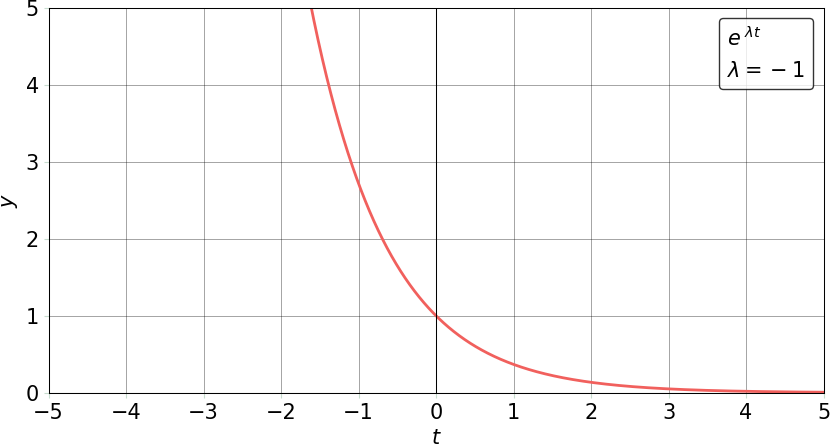
\includegraphics[width=0.4\textwidth]{Exponential Decay/Exact with -1.png}
\end{center}
\end{multicols}

\newpage
\subsection{Numerical Method: Forward Euler}

\par We will now consider a simple numerical method applied to the exponential decay problem.
The Forward Euler method is a first-order numerical method for solving ODEs with a given initial condition.
Its algorithm can be defined as follows:
\[ y(t_{j+1}) = y(t_j) + h y'(t_j)\]
Or equivalently:
\[ y_{j+1} = y_j + h \phi(t_j, y_j)\]
Where $h$ is the time step and $y_j$ is the numerical solution at time $t_j$.

\par For the exponential decay problem, the Forward Euler method can be written as:
\[ y_{j+1} = y_j + h \lambda y_j \quad \text{where} \quad y_0 = 1\]
This gives us the following algorithm:
\[ y_{j+1} = (1 + h \lambda) y_j\]
This gives an approximation of the exact solution at time $t_j$ as follows:
\[ y_{j} \approx {(1 + h \lambda)}^j y_0\]

\par We can see that the Forward Euler method is stable if $|1 + h \lambda| < 1$; both the exact solution and our approximation will decay to zero as $t \rightarrow \infty$.
The stability is dependent on the time step $h$ and the value of $\lambda$.
We can write this as $s(\lambda, h) = 1 + h \lambda$.
By analysing $s$ for different values of $\lambda$ and $h$, we can infer the stability of the Forward Euler method for the exponential decay problem.
We call $s$ the \term{stability function} of the Forward Euler method.



\subsection{The Stability Function and corresponding Stability Region}
\par By the same methodology, we can define the stability function for any numerical method:\\
Write the algorithm in the form $y_{j+1} = s(\lambda, h) y_{j}$.\\
$s(\lambda, h)$ is the \term{stability function} of the numerical method with a time step $h$.\\
\textbf{Note:} This is equivalent to $y_{j} = {s(\lambda,h)}^{j} y_0$

\par The \term{stability region} of a numerical method is the set $S = \Big\{ (\lambda, h) \;\Big|\; |s(\lambda, h)| < 1\Big\}$\\
This follows from the definition of stability for our exponential decay problem; a method is stable if the numerical solution decays to zero as $t \rightarrow \infty$.\\
Clearly, $y_{j} = {s(\lambda,h)}^{j} y_0$ will decay to zero as $j \rightarrow \infty$ if $|s(\lambda, h)| < 1$.

\subsubsection{Stability Region for Euler's Forward Method}
\begin{multicols}{2}
\vspace*{\fill}

Euler's Forward Method has the stability function
\[s(\lambda, h) = 1 + \lh\]
The corresponding stability region is 
\[S = \Big\{ (\lambda, h) \;\Big|\; |1 + \lh| < 1\Big\}\]
We can see this region plotted in red on the right; a unit circle centred at $-1$.\\
For a given $\lambda \in \bC$, the method is stable for any step-size $h \in \bR$ such that $|1 + \lh| < 1$.\\
Expanding $\lambda = a + bi$, we get the restriction
\[|1 + (a + bi)h| < 1 \quad \implies \quad a^2h^2 + 2ah + b^2h^2 < 0\]
As $a, b$ and $h \in \bR$, $(a^2 +b^2)h^2 > 0$\\
$\implies 2ah < 0$ with $|2ah| > (a^2 + b^2)h^2$

\vspace*{\fill}
\columnbreak{}
\begin{center}
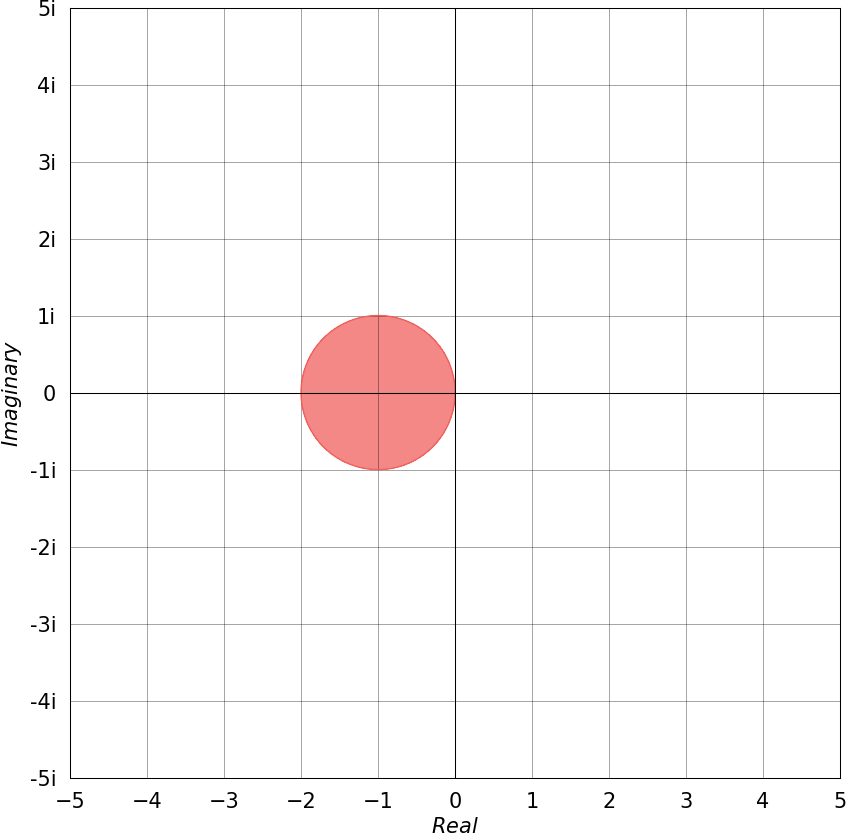
\includegraphics[width=0.49\textwidth]{Stability Regions/Graphs/Real 1-Step/Euler's Forward.png}
\end{center}
\end{multicols}

\subsubsection{Stability Region for Euler's Backward Method}
\begin{multicols}{2}
\begin{center}
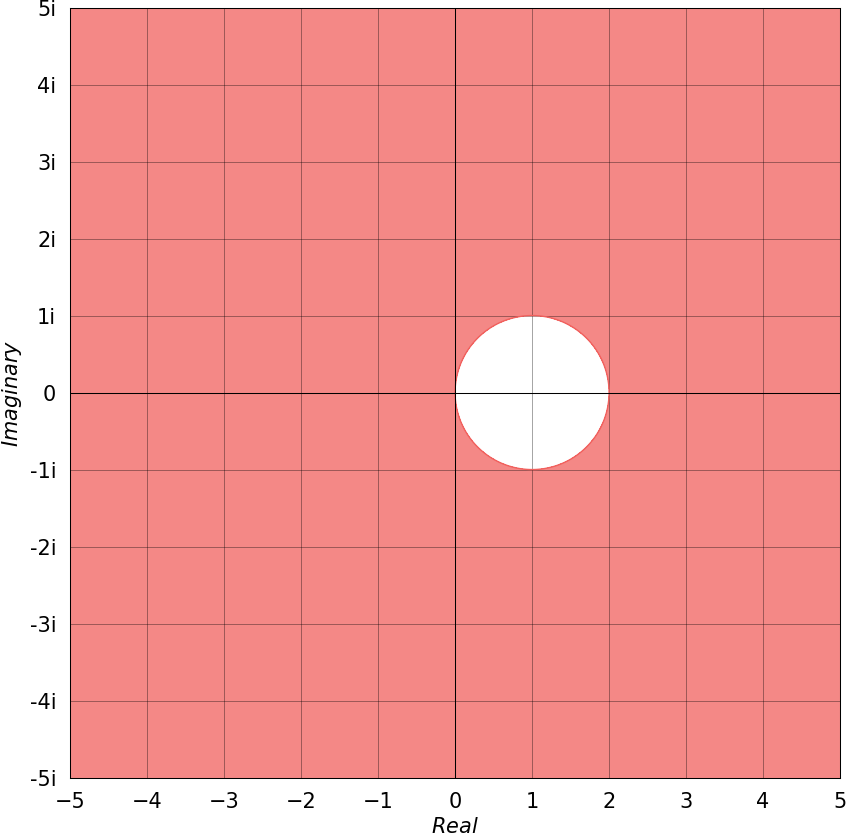
\includegraphics[width=0.49\textwidth]{Stability Regions/Graphs/Real 1-Step/Euler's Backward.png}
\end{center}
\columnbreak{}
\vspace*{\fill}

Euler's Backward Method can be written as
\[y_{j+1} = y_j + h.\phi(t_{j+1}, y_{j+1})\]
\[\implies y_{j+1} = y_j + h(\lambda y_{j+1}) \implies y_{j+1} = \frac{1}{1 - \lh}y_j\]
Thus, the stability function is
\[s(\lambda, h) = \frac{1}{1 - \lh}\]
The corresponding stability region is
\[S = \Big\{ (\lambda, h) \;\Big|\; \left|\frac{1}{1 - \lh}\right| < 1\Big\}\]
This is plotted in red on the left; the region outside a unit circle centred at $1$.\\
The white region of instability is exactly the stability region for Euler's Forward Method, flipped about Imaginary axis.\\
\vspace*{\fill}
\end{multicols}

\subsubsection{Stability Region for Runge-Kutta 4}
\begin{multicols}{2}
\vspace*{\fill}

Runge-Kutta 4 can be written as
\[y_{j+1} = y_j + \frac{h}{6}(k_1 + 2k_2 + 2k_3 + k_4)\]
Where
\begin{flalign*}
	k_1 &= \phi(t_j, y_j) \quad &k_2 = \phi(t_j + \frac{h}{2}, y_j + \frac{h}{2}k_1) && \\
	k_3 &= \phi(t_j + \frac{h}{2}, y_j + \frac{h}{2}k_2) \quad &k_4 = \phi(t_j + h, y_j + hk_3) &&
\end{flalign*}
For the Exponential Decay Problem, we get
\[y_{j+1} = (1 + \lh + \frac{{(\lh)}^2}{2} + \frac{{(\lh)}^3}{6} + \frac{{(\lh)}^4}{24})y_j\]
The stability function is $s(\lambda, h) = \sum\limits_{m=0}^{4}\frac{{(\lh)}^m}{m!}$\\
The corresponding stability region is
\[S = \Big\{ (\lambda, h) \;\Big|\; \left|\sum\limits_{m=0}^{4}\frac{{(\lh)}^m}{m!}\right| < 1\Big\}\]

\vspace*{\fill}
\columnbreak{}
\begin{center}
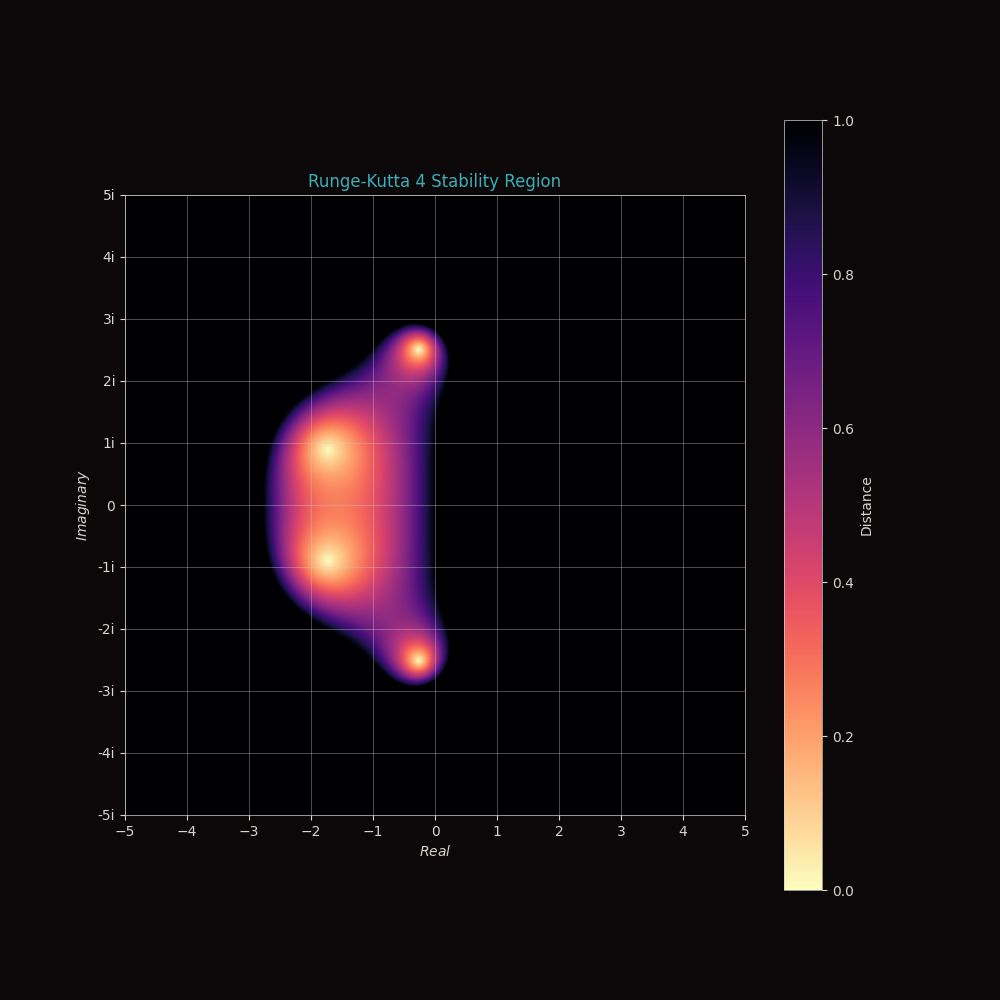
\includegraphics[width=0.49\textwidth]{Stability Regions/Graphs/Real 1-Step/Runge-Kutta 4.png}
\end{center}
\end{multicols}

\subsection{Interpretation of Stability Regions}
\par In the first graph, shaded in grey, is the region of stability for Runge-Kutta 4.\\
This region is the set of $\lh$ values for which the method is stable.\\

\par In all other graphs, in black, is a plot of the exact solution to the Exponential Decay Problem for a given $\lambda$.
For this curve to appear smooth, a step-size in t of $h = \frac{1}{1000}$ was used.\\

\par As we have fixed $h$, the stability region gives the set of values $\frac{\lambda}{1000}$ for which the method is stable.\\
From this we can derive stable $\lambda$ values.

\par Highlighted on the left are $n$ coloured points, representing $n$ different values of $\frac{\lambda}{1000}$.
The green point is $-1$, and sits inside the stability region.
This tells us that the method is stable for $\lambda = -1000$.\\
We can see this on the right, as the green curve of RK4 with $\lambda = -1000$ decays to zero and closely follows the exact solution in black.\\

MORE DETAIL HERE\\


\subsection{Numerical Method: 2-step Abysmal Kramer-Butler Method}

\par This method was designed to be unstable for the sake of demonstration.\\
The algorithm is as follows:
\[y_{j+1} = y_{j-1} + h(4\phi(t_j,y_j)-2\phi(t_{j-1},y_{j-1}))\]
As we know the exact solution to our Exponential Decay problem is $y(t) = e^{\lambda t}$, we know $\phi(t,y) = \lambda y$.\\
This gives:\\
\[y_{j+1} = y_{j-1} + h(4\lambda y_j - 2\lambda y_{j-1})\]
Simplified:\\
\[y_{j+1} = 4\lh y_j + (1-2\lh) y_{j-1}\]
%FURTHER DERIVATION ON WHITEBOARD - Aim: Get method in terms of $y_{j}$, $y_1$ and $y_0$ only.\\
